%%
%% This is file `sample-sigconf.tex',
%% generated with the docstrip utility.
%%
%% The original source files were:
%%
%% samples.dtx  (with options: `sigconf')
%% 
%% IMPORTANT NOTICE:
%% 
%% For the copyright see the source file.
%% 
%% Any modified versions of this file must be renamed
%% with new filenames distinct from sample-sigconf.tex.
%% 
%% For distribution of the original source see the terms
%% for copying and modification in the file samples.dtx.
%% 
%% This generated file may be distributed as long as the
%% original source files, as listed above, are part of the
%% same distribution. (The sources need not necessarily be
%% in the same archive or directory.)
%%
%%
%% Commands for TeXCount
%TC:macro \cite [option:text,text]
%TC:macro \citep [option:text,text]
%TC:macro \citet [option:text,text]
%TC:envir table 0 1
%TC:envir table* 0 1
%TC:envir tabular [ignore] word
%TC:envir displaymath 0 word
%TC:envir math 0 word
%TC:envir comment 0 0
%%
%%
%% The first command in your LaTeX source must be the \documentclass command.
\documentclass[sigconf]{acmart}

% To remove "ACM Reference Format" section
\settopmatter{printacmref=false}
\renewcommand\footnotetextcopyrightpermission[1]{} % removes conference footnote

%%
%% \BibTeX command to typeset BibTeX logo in the docs
\AtBeginDocument{%
  \providecommand\BibTeX{{%
    \normalfont B\kern-0.5em{\scshape i\kern-0.25em b}\kern-0.8em\TeX}}}

%% Rights management information.  This information is sent to you
%% when you complete the rights form.  These commands have SAMPLE
%% values in them; it is your responsibility as an author to replace
%% the commands and values with those provided to you when you
%% complete the rights form.
% \setcopyright{acmcopyright}
% \copyrightyear{2025}
% \acmYear{2025}
% \acmDOI{10.1145/3524844.3528051}
% %% These commands are for a PROCEEDINGS abstract or paper.
% \acmConference[Software Engineering Research Project 2024-2025]{}{2025}{Milan, MI, Italy}

% \acmConference[Woodstock '18]{Woodstock '18: ACM Symposium on Neural
%   Gaze Detection}{June 03--05, 2018}{Woodstock, NY}
% \acmBooktitle{Woodstock '18: ACM Symposium on Neural Gaze Detection,
%   June 03--05, 2018, Woodstock, NY}
% \acmPrice{15.00}
% \acmISBN{978-1-4503-XXXX-X/18/06}


%%
%% Submission ID.
%% Use this when submitting an article to a sponsored event. You'll
%% receive a unique submission ID from the organizers
%% of the event, and this ID should be used as the parameter to this command.
%%\acmSubmissionID{123-A56-BU3}

%%
%% The majority of ACM publications use numbered citations and
%% references.  The command \citestyle{authoryear} switches to the
%% "author year" style.
%%
%% If you are preparing content for an event
%% sponsored by ACM SIGGRAPH, you must use the "author year" style of
%% citations and references.
%% Uncommenting
%% the next command will enable that style.
%%\citestyle{acmauthoryear}

\usepackage{algorithm} 
\usepackage{algpseudocode} 
\usepackage{makecell} 
\usepackage{xspace} 
\usepackage[nocomma]{optidef}
% don't add package ulem, otherwise bib will be underlined
% \usepackage{ulem} 
\usepackage{enumitem}
\usepackage{graphicx}
\usepackage{subcaption}
\usepackage{multirow}
\usepackage{balance}

%%
%% end of the preamble, start of the body of the document source.
\acmBooktitle{Software Engineering Research Project 2024-2025}
\begin{document}

\newcommand{\dav}[1]{\textcolor{cyan}{\textbf{[DH] #1}}}
\newcommand{\nic}[1]{\textcolor{green}{\textbf{[NS] #1}}}
\newcommand{\bea}[1]{\textcolor{orange}{\textbf{[BZ] #1}}}

%%
%% The "title" command has an optional parameter,
%% allowing the author to define a "short title" to be used in page headers.
\title[Evaluation of AI agents using the Carla Leaderboard Evaluator]{Evaluation of AI agents using the Carla Leaderboard Evaluator}

\author{Niccolò Salvi}
\email{niccolo1.salvi@mail.polimi.it}
\affiliation{
  \institution{Politecnico di Milano}
  \department{Dipartimento di Elettronica, Informazione e Bioingegneria}
  \city{Milan}
  \country{Italy}
}

\author{Beatrice Zani}
\email{beatrice.zani@mail.polimi.it}
\affiliation{
  \institution{Politecnico di Milano}
  \department{Dipartimento di Elettronica, Informazione e Bioingegneria}
  \city{Milan}
  \country{Italy}
}

%%
%% The abstract is a short summary of the work to be presented in the
%% article.
\begin{abstract}
This paper presents a comparative evaluation of AI-based autonomous driving agents, InterFuser and TransFuser, using the CARLA Leaderboard Evaluator. Both models are state-of-the-art sensor fusion architectures designed to enhance urban autonomous navigation. The primary objective of this study is to assess and contrast their performance and behavioral characteristics in diverse urban driving scenarios. Leveraging the standardized CARLA Leaderboard metrics, we systematically analyze aspects such as route completion, infraction rates, and driving safety. Additionally, we reviewed qualitative video footage of the agents' driving sessions to identify and characterize unusual or problematic behaviors not captured by quantitative metrics. The results contribute to the broader effort of benchmarking autonomous driving policies in simulation and support informed development of future sensor fusion architectures.
\end{abstract}

% \ccsdesc[300]{Theory of computation~Scheduling algorithms}
% \ccsdesc[300]{Computing methodologies~Distributed computing methodologies}
% \ccsdesc[300]{Computer systems organization~Distributed architectures}

%%
%% Keywords. The author(s) should pick words that accurately describe
%% the work being presented. Separate the keywords with commas.
\keywords{Imitation Learning, Autonomous Driving, Transformer, Sensor Fusion, CARLA simulator, InterFuser, TransFuser}

%% information and builds the first part of the formatted document.
\maketitle

\section{Introduction}
\label{sec:intro}

Autonomous driving is one of the most ambitious challenges in artificial intelligence, with the potential to revolutionize transportation. A key aspect of this field is the development and evaluation of driving agents capable of making real-time decisions based on multi-modal sensor inputs, such as cameras, LiDAR, and route planning data. Accurately benchmarking these agents is essential for pushing the field forward and ensuring their safe, reliable operation in complex urban environments. Simulation platforms like CARLA (Car Learning to Act) offer a standardized and controllable environment to evaluate such systems.
    
Within this space, TransFuser and InterFuser are two leading AI driving agents designed to tackle the sensor fusion problem. Both models have achieved strong performance on the CARLA Leaderboard, which ranks agents based on their behavior in realistic driving scenarios. However, while leaderboard metrics such as route completion and infraction scores provide useful performance indicators, they don’t always capture the full picture—especially when agents behave in strange or unexpected ways. This work seeks not only to compare these two agents in terms of traditional metrics such as route completion and infractions but also to investigate the underlying causes of unusual behaviors observed during their operation.

This study evaluates existing pre-trained end-to-end state-of-the-art agents such as TransFuser and InterFuser within the CARLA simulation environment using the CARLA Leaderboard framework. The agents are used as-is, without any retraining or modification. Our focus is on comparing their performance under identical conditions and conducting a qualitative investigation into their behavior. Special attention is given to identifying instances where the agents exhibit unusual or flawed decision-making and attempting to determine the underlying causes by examining the simulation context, sensor inputs, and environmental factors.
\section{Background}
\label{sec:background}

This section provides the necessary background for our analysis. It covers the primary strategies in autonomous driving development, explains the importance of virtual simulation and standardized benchmarking for research, and introduces the specific models examined in this study.

\subsection{Autonomous Driving Agents}
In recent years, autonomous driving has experienced remarkable advancements thanks to companies such as Tesla and Waymo, which adopt distinct strategies to achieve fully autonomous vehicles. Tesla utilizes a camera-based approach known as \textit{Tesla Vision}~\footnote{See Tesla Support, "Replacing Ultrasonic Sensors with Tesla Vision" Dec 2024.}, relying solely on RGB cameras and artificial intelligence without incorporating LiDAR or radar sensors. This vision-based approach aims to emulate human perception, employing neural networks to interpret images and make driving decisions. Tesla's long-term goal is achieving SAE Level 5 autonomy, which implies complete autonomous driving capability under any conditions without human intervention.

Conversely, Waymo\footnote{See Waymo, "Self-Driving Car Technology for a Reliable Ride - Waymo Driver" 2024; Automotive Dive, "A look inside the sixth-generation Waymo Driver" 2024.} adopts a comprehensive sensor suite including RGB cameras, radar, and LiDAR sensors. This multi-sensor integration provides robust three-dimensional perception, enhancing the safety and reliability of the autonomous system. Waymo has already deployed autonomous ride-hailing services in selected U.S. cities such as Phoenix and San Francisco, continuously expanding its autonomous fleet. Both companies share the ultimate vision of transforming mobility by reducing traffic accidents and increasing urban transportation efficiency.

\subsection{CARLA Simulator}
CARLA (Car Learning to Act)~\cite{dosovitskiy2017carlaopenurbandriving} is an open-source simulator explicitly developed to support autonomous driving research, development, training, and validation. It provides a realistic virtual urban environment populated with vehicles, pedestrians, traffic signals, and varying weather conditions. Employing virtual simulations like CARLA has significant advantages over real-world testing. Virtual environments ensure safety by allowing testing of dangerous scenarios without risks to individuals or property. Additionally, simulations offer greater efficiency, enabling rapid execution of numerous tests at reduced costs. The controlled environment provided by CARLA allows precise replication of specific conditions, facilitating systematic comparisons and accurate performance evaluations of various autonomous driving algorithms. Consequently, CARLA has emerged as an essential tool within autonomous driving research.

\subsection{CARLA Autonomous Driving Leaderboard}
The CARLA Autonomous Driving Leaderboard~\footnote{CARLA Autonomous Driving Leaderboard. Available at: \url{http://leaderboard.carla.org}} is an evaluation platform specifically designed to compare the performance of diverse autonomous driving agents within the CARLA simulator. Through standardized scenarios, agents are assessed on multiple aspects such as adherence to traffic rules, obstacle management, and navigation capability. Annually, a global competition organized by the CARLA community invites participation from universities, research institutions, and industry players to foster innovation and establish benchmarks in the field.

Models such as TransFuser~\cite{chitta2022transfuserimitationtransformerbasedsensor} and InterFuser~\cite{shao2022safetyenhancedautonomousdrivingusing} have actively participated in these competitions, notably in the 2021 and 2022 editions, respectively, achieving significant results and influencing advancements in the domain. The CARLA Leaderboard thus serves as a crucial standard for evaluating and benchmarking autonomous driving agents, accelerating progress and facilitating collaborative development within the research community.

\subsubsection{Evaluation Metrics}
The CARLA Leaderboard employs a comprehensive set of metrics to assess the performance of autonomous driving agents. The primary metric is the Driving Score, denoted as \( D_i \), which evaluates an agent's ability to complete routes while adhering to traffic rules and avoiding infractions. It is calculated as the product of the Route Completion \( R_i \) and the Infraction Penalty \( P_i \):

\[ D_i = R_i \times P_i \]

Here, \( R_i \) represents the percentage of the route completed by the agent, with a maximum value of 100\%, and \( P_i \) is a coefficient reflecting the penalties incurred due to infractions, ranging from 0 to 1.

The Infraction Penalty \( P_i \) is determined by aggregating the penalties from various infractions committed during the route. Each infraction type has an associated penalty coefficient \( p_j \), and the overall penalty is computed as:

\[ P_i = \prod_j p_j^{n_j} \]

where \( n_j \) is the number of times infraction \( j \) occurred. This multiplicative approach ensures that repeated infractions have a compounding negative effect on the driving score.

Infractions are categorized based on their severity, with corresponding penalty coefficients. For instance, collisions with pedestrians have a penalty coefficient of 0.50, collisions with vehicles 0.60, collisions with static objects 0.65, running a red light 0.70, failing to yield to emergency vehicles 0.70, and running a stop sign 0.80. Additional penalties are applied for scenario timeouts (0.70), failure to maintain minimum speed (up to 0.70), and off-road driving, which reduces the route completion percentage accordingly.

Furthermore, certain events can lead to the termination of a simulation run. These include deviating more than 30 meters from the assigned route, the agent being inactive for 180 simulation seconds, simulation timeouts due to communication issues, exceeding the maximum allowed time for a route, and errors within the agent's code. In such cases, the route is marked as failed, and the simulation proceeds to the next route.

\subsection{Overview of Studied Models}
The models analyzed in this study, InterFuser and TransFuser, have each represented a significant milestone in the evolution of autonomous driving agents, particularly within the CARLA simulation environment.

\subsubsection{InterFuser}
InterFuser~\cite{shao2022safetyenhancedautonomousdrivingusing} is a neural network-based model leveraging deep learning, designed to integrate interpretable intermediate representations with direct end-to-end control. It combines inputs from RGB cameras and LiDAR sensors to produce two primary outputs: a sequence of waypoints representing the desired future trajectory of the vehicle, and an object density map encoding spatial and dynamic information about surrounding agents such as vehicles, pedestrians, and cyclists. Additionally, InterFuser predicts traffic rules such as traffic light states and stop signs. This integration enables the implementation of a safety controller that considers predicted future trajectories of surrounding objects to plan safe maneuvers.

In addition to generating a sequence of waypoints, InterFuser outputs an object density map ($M$), which represents the space around the vehicle as a grid of $(1,\text{m}) \times (1,\text{m})$ cells. Each cell encodes seven features that describe the presence and potential state of nearby objects such as vehicles, pedestrians, and cyclists: existence probability, offset from the cell center, bounding box size, heading, and object velocity. To detect the presence of an object in a cell of the map, two probability thresholds are applied. However, to assess the safety of the predicted trajectory, the controller employs a tracking system that records the motion history of objects surrounding the vehicle. It then estimates their future positions by applying a moving average over the observed dynamics.

\subsubsection{TransFuser}
TransFuser~\cite{chitta2022transfuserimitationtransformerbasedsensor} relies on a transformer-based architecture for multi-sensor fusion. It processes RGB images and LiDAR data using dedicated encoders and then fuses the resulting feature maps through cross-attention mechanisms. The model outputs future waypoints in the Bird’s Eye View plane, which are used by a PID controller to derive steering and acceleration commands. In addition, TransFuser performs auxiliary tasks such as semantic segmentation and object detection, improving the interpretability and generalization of the learned policies.

The original TransFuser paper introduces several architectural variants that explore different approaches to multi-modal sensor fusion. These variants differ primarily in how they combine RGB and LiDAR information, ranging from attention-based mechanisms to geometric projections and simplified fusion strategies. We describe these variants below to provide a comprehensive overview of the TransFuser family.

\paragraph{LatentTF} LatentTF was explicitly introduced in the original TransFuser paper to study the effect of removing LiDAR data. It shares the same Transformer backbone and prediction objectives but uses static positional encoding in place of real-world geometric input from LiDAR, offering a clean ablation for sensor dependence. that removes the explicit LiDAR input and instead relies on a fixed latent positional encoding to guide the fusion process. This architectural modification reduces computational complexity, making the model more lightweight, but at the expense of robustness in geometrically challenging scenes or under degraded visibility. Despite this, LatentTF retains the core Transformer-based structure and learning objectives of TransFuser, making it suitable for benchmarking the impact of sensor reduction on driving performance.

\paragraph{Late Fusion} Late Fusion is a variation of TransFuser in which RGB and LiDAR features are extracted independently using standard encoders, and then combined through simple element-wise summation rather than via attention mechanisms. While computationally efficient, this approach lacks the rich inter-modal interactions provided by transformers, limiting its expressiveness in complex driving scenarios.

\paragraph{Geometric Fusion} Geometric Fusion replaces the attention-based fusion of TransFuser with projection-based feature integration. It unprojects LiDAR BEV cells into 3D space, samples LiDAR points, and reprojects them into the image plane to aggregate visual features. These are fused through a multi-layer perceptron and combined with LiDAR features at multiple scales. This approach emphasizes geometrically grounded alignment but increases implementation complexity.

\paragraph{Model Selection}
For this study, we selected three models for comparative analysis: InterFuser, TransFuser (main model), and LatentTF. InterFuser and TransFuser were chosen primarily due to their widespread adoption and established performance benchmarks in the autonomous driving literature, making them representative baselines for evaluating multi-modal fusion approaches. 
In this project, LatentTF was included in the analysis to investigate how the absence of direct LiDAR data would impact the model’s behavior, particularly in challenging scenarios such as high-traffic environments and creeping situations. The authors of TransFuser describe a \textit{creeping mechanism}, triggered when the agent remains stationary for an extended period, which is designed to push the vehicle slightly forward to prevent deadlocks. During evaluations, the hypothesis was that issues in creeping behavior could be related to LiDAR data processing, and thus, there was an interest in assessing whether LatentTF, being solely vision-based, would perform differently under the same conditions. Geometric Fusion and Late Fusion models were excluded from this analysis. While important for understanding early fusion techniques, they are less relevant to our core research question, which focuses on comparing the advanced attention-based fusion of TransFuser with the intermediate representation approach of InterFuser, and analyzing the specific impact of LiDAR data via LatentTF.
\section{Problem Statement}
\label{sec:problem}

Autonomous driving benchmarks, like the CARLA Leaderboard, provide essential quantitative scores but often fail to explain why an agent fails. For example, an agent might receive a low Route Completion score for getting stuck, but the metric itself does not reveal the underlying cause. For instance, an autonomous vehicle might remain stationary, failing to complete its route due to an obstacle improperly placed on the sidewalk, rather than due to an actual shortcoming in the model's decision-making capabilities. Was it a perception failure, an overly conservative planner, or a simulation artifact?

We conduct a deep, qualitative investigation into the behavior of three state-of-the-art models: InterFuser, TransFuser and LatentTF. The primary challenge tackled by this study is that even top-performing agents exhibit subtle yet critical failures that are not fully captured by scores alone. These problematic behaviors can be caused by a variety of sources, including complex interactions with other vehicles, strict adherence to traffic rules under ambiguous conditions, or challenging environmental factors like poor lighting.

This study critically examines the performance of these agents in a controlled CARLA environment to identify and diagnose specific failure modes. We aim to understand the root causes of these issues by analyzing the simulation context, sensor inputs, and the models' decision-making processes.
\section{Methodology}
\label{sec:methodology}

This section details the systematic approach used to evaluate the InterFuser and TransFuser agents. We outline the experimental environment, the necessary software adaptations to run the agents on a modern toolchain, and the protocol followed for both quantitative and qualitative analysis.

\subsection{Experimental Setup}
\label{subsec:setup}

Our evaluation was conducted within a standardized environment to ensure the reproducibility of our findings.

\noindent\textbf{Software Environment:} The experiments were run using CARLA simulator version 0.9.14 and Python 3.8. This represents an update from the original agents' environments (CARLA 0.9.10 and Python 3.7), necessitating the code adaptations detailed below (\autoref{subsec:config}.

\noindent\textbf{Hardware:} All simulations were run on a workstation equipped with a dual Intel Xeon E5-2696 V2 CPU, 144 GB of RAM, and an NVIDIA GeForce RTX 3080ti GPU.

\noindent\textbf{Agents:} We used the official, pre-trained weights for InterFuser and TransFuser (including LatentTF) without any retraining. The models were evaluated ``as-is'' to analyze their out-of-the-box performance.

\subsection{Agent Configuration and Adaptation}
\label{subsec:config}

Key adaptations for both agents involved resolving dependency conflicts with visualization libraries like \texttt{matplotlib} and \texttt{open3d}, and fixing runtime errors caused by deprecated CARLA API calls, most notably by replacing \texttt{GlobalRoutePlannerDAO} with the current \texttt{GlobalRoutePlanner} class. We also installed specific versions of deep learning packages, such as \texttt{torch-scatter} and \texttt{mmcv-full}, to ensure compatibility with our toolchain. For InterFuser, we further modified the agent's code to save sensor images during simulation, which was essential for our qualitative analysis. These modifications were necessary to achieve stable and reliable execution of the agents in our experimental setup.

All changes have been documented and published on online repositories.\footnote{InterFuser Fork, \url{https://github.com/NiccoloSalvi/InterFuser-Carla0914}}\textsuperscript{,}\footnote{TransFuser Fork, \url{https://github.com/NiccoloSalvi/TransFuser-Carla0914}}

\subsection{Metrics}
\label{subsec:metrics}
Our evaluation methodology combined quantitative metrics with in-depth qualitative analysis to provide a comprehensive assessment of agent performance.

\noindent\textbf{Quantitative Evaluation:} We executed the agents on the official CARLA Leaderboard benchmark, running the scenarios and routes publicly available at the following link\footnote{\url{https://github.com/opendilab/InterFuser/tree/main/leaderboard/data/42routes}}.
Specifically, for the InterFuser agent, we performed two repetitions for each available route and scenario from the provided set. For the TransFuser (TF) agent, in addition to approximately twenty scenarios selected from the CARLA Leaderboard, we also executed several routes specifically from \textit{Town05}, using the evaluation routes accessible at this link\footnote{\url{https://github.com/opendilab/InterFuser/tree/main/leaderboard/data/evaluation_routes}}.
For each scenario, we collected the standard metrics, including the Driving Score, Route Completion, and a detailed breakdown of infractions (e.g., collisions, running red lights, stop sign violations).

\noindent\textbf{Qualitative Analysis:} The primary goal of this study was to understand the \textit{reasons} behind the quantitative scores. To achieve this, we conducted a systematic review of video recordings and saved images from the simulation runs. This process involved identifying failure patterns, where we manually logged recurring problematic behaviors, such as premature stopping, getting blocked by obstacles, and unsafe ``creeping'' maneuvers.
Additionally, we dignased the root cause of the failure, where, for each identified failure, we analyzed the corresponding sensor inputs (RGB camera, LiDAR BEV) and model outputs (predicted waypoints, object detection) to hypothesize the root cause.
Finally, we performed a comparative analysis. We compared the behaviors of InterFuser, TransFuser, and LatentTF in identical scenarios to understand how architectural and sensor differences influenced their decision-making.

\section{Results}
This section outlines the models used for experimentation and presents a critical analysis of their performance. Our methodology combines a qualitative assessment of agent behavior in carefully selected critical scenarios with a quantitative evaluation based on standard metrics provided by the CARLA simulator.

\subsection{Analysis of Agent Behavior}
To complement our findings, we employed a structured approach to qualitatively analyze agent behavior. During simulation runs, we recorded video footage and periodically saved sensor data, including RGB camera views, LiDAR BEV outputs and density maps. Each simulation session was reviewed manually to identify and document behavioral failures.

The review process was done by both of us, with each video analyzed independently by both team members to ensure consistency and manageability. Following the individual reviews, we discussed about our observations and defined a set of recurring failures.

To communicate the prevalence of each failure type, we introduced the following frequency labels:
\begin{itemize}
    \item\textbf{Frequent:} Occurred in more than 5 distinct episodes across the evaluation set.
    \item\textbf{Occasional:} Occurred between 3 and 6 times.
    \item\textbf{Rare:} Occurred once or twice.
\end{itemize}
For each failure, we attempted to diagnose the root cause by reviewing corresponding sensor inputs, model outputs and code implementation. This analysis was supplemented by consulting open issues and community discussions in the official GitHub repositories and forums for CARLA\footnote{\url{https://github.com/carla-simulator/carla}}, TransFuser\footnote{\url{https://github.com/autonomousvision/transfuser}} and InterFuser\footnote{\url{https://github.com/opendilab/InterFuser}}.

Our analysis of the driving agents in the CARLA simulator revealed several recurring failure modes. While both models performed well on standard metrics, a closer look at their behavior uncovered specific, repeatable issues that are not immediately obvious from quantitative scores alone. These problems highlight systemic weaknesses in how the agents perceive their environment, interpret rules, and interact with other vehicles.

These issues span from perception-related deficits to suboptimal decision-making heuristics and limitations in motion planning. The most prominent problems observed include: (i) premature stopping at intersections or traffic lights, where the vehicle halts significantly before the designated stop line, thereby impairing its ability to perceive signal changes or proceed through intersections smoothly; (ii) failure to come to a complete stop at stop signs, leading to traffic rule violations; (iii) a tendency to remain indefinitely blocked in the presence of nearby static or dynamic obstacles due to overly conservative safety constraints; (iv) severe degradation of performance under low-light conditions, often manifesting as erratic behavior or misinterpretation of critical environmental cues; (v) unreliable or unsafe creeping behavior, where forced forward movement in stationary conditions frequently results in collisions, particularly in densely populated urban scenarios; and (vi) inadequate throttle control on upward slopes, where the vehicle lacks the torque to initiate motion, resulting in indefinite idling or rollback.

It is important to note that while these problems were observed in the two models, their root causes are not exclusively attributed to neural network deficiencies. Instead, some issues may be caused by other interconnected components of the autonomous driving system, such as inaccuracies in the prediction of movements of nearby subjects.
These limitations, although heterogeneous in manifestation, collectively reveal systemic weaknesses in perception fusion, behavior arbitration, and predictive modeling. They also highlight the inadequacy of relying solely on rigid heuristics or rule-based fallbacks in scenarios that demand adaptive and context-aware decision-making. 

An overview of the problems encountered can be found in Table \ref{tab:failure_modes}, which summarizes these problems, indicating their frequency and the specific model in which they were observed.

\begin{table}[t]
    \small
    \centering
    \caption{Summary of Common Failure Modes Across Models}
    \label{tab:failure_modes}
    \resizebox{\columnwidth}{!}{%
    \begin{tabular}{@{}lll@{}}
        \toprule
        \textbf{Problem} & \textbf{Model(s)} & \textbf{Frequency} \\
        \midrule
        \textbf{P1.} Premature Stopping at Traffic-Controlled Intersections & InterFuser & Frequent \\
        \textbf{P2.} Agent freezes when obstacle are nearby & InterFuser & Occasional \\
        \textbf{P3.} Agent Struggles in Very Dark Conditions & InterFuser & Frequent \\
        \textbf{P4.} Car does not full stop at stop sign & TransFuser & Occasional \\
        \textbf{P5.} Cannot see traffic lights turning green & TransFuser & Rare \\
        \textbf{P6.} The problem of creeping & TransFuser & Frequent \\
        \textbf{P6.} The problem of creeping & LatentTF & Frequent \\
        \bottomrule
    \end{tabular}
    }
\end{table}

\subsection{P1. Premature Stopping at Traffic-Controlled Intersections}\label{P1}
\noindent\textbf{Issue.} We observed that the InterFuser agent frequently underestimates its actual distance from traffic lights, often stopping well before the designated stop line or behind vehicles already waiting at the light, even when there is ample space ahead. While this behavior does not directly impact the leaderboard score, it is unrealistic and would be unacceptable in real-world driving scenarios. Stopping too early at intersections can cause abnormal queuing and traffic congestion, thereby increasing the risk of hazardous or difficult situations for other road users.
In some cases, the agent begins to move when the light turns green, but because it had stopped too far from the intersection, it fails to reach the stop line in time and is forced to stop again at the next red light—ultimately having to wait for an additional green cycle.

\noindent\textbf{Reason.} The key cause of this problem is that the agent has issues in accurately estimating two critical distances: the distance to the relevant traffic light controlling its movement, and the distance to the actual intersection. Inaccurate estimation of these distances leads the vehicle to halt prematurely. This behavior has also been analyzed in this issue from the official repository of the agent\footnote{\url{https://github.com/opendilab/InterFuser/issues/39}}.

\noindent\textbf{Proposed Solution.} Some users in the online discussion have suggested mitigating this issue by reducing the red-light detection threshold, thereby increasing the agent’s sensitivity and enabling it to recognize red lights only at closer proximity. However, this approach risks introducing numerous false positives (instances where more red lights are detected than actually exist) ultimately degrading the agent’s behavior and making its stopping decisions even less reliable.
A possible solution could be for the agent to use HD map data—which contains exact stop line positions and traffic light locations—to calculate the correct stopping distance relative to its current pose and route. This would eliminate the need to rely only on image-based depth estimation, which is more prone to error as we have observed.

\begin{figure}[htbp]
    \centering
    \begin{subfigure}[b]{0.45\textwidth}
        \centering
        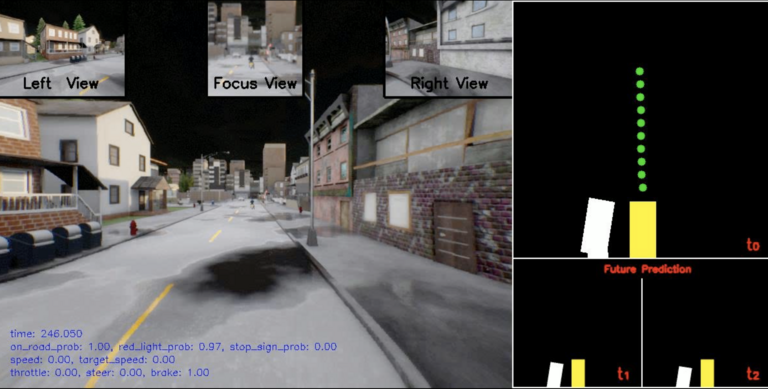
\includegraphics[width=\columnwidth]{images/RS10_R0_firstStop.png}
        \Description{The InterFuser agent stops prematurely at a significant distance before the intersection and the stop line.}
        \caption{Initial premature stop of the InterFuser agent at a traffic-controlled intersection. The ego vehicle incorrectly halts well before the designated stop line, due to inaccurate estimation of its distance to the relevant traffic signal and the intersection. Despite clear and sufficient road space ahead, this overly cautious behavior could lead to abnormal queueing and potential traffic congestion.}
        \label{fig:RS10_premature_first_stop}
    \end{subfigure}
    \hfill
    \begin{subfigure}[b]{0.45\textwidth}
        \centering
        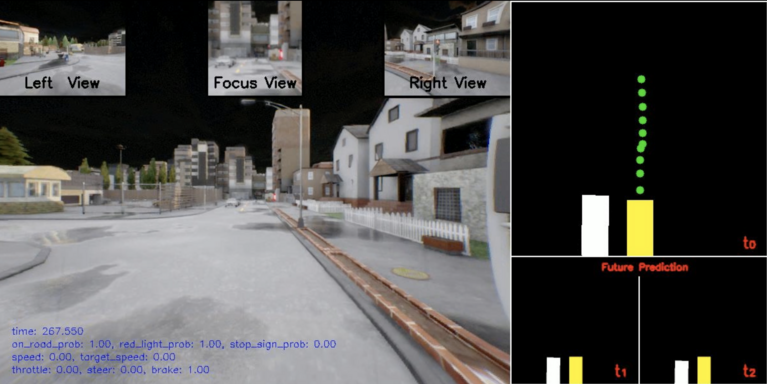
\includegraphics[width=\columnwidth]{images/RS10_R0_secondStop.png}
        \Description{The InterFuser agent makes a second stop, closer to the intersection, after initially halting prematurely.}
        \caption{Second stop of the InterFuser agent, closer to the intersection. Due to its previous premature halt, when the traffic light turns green, the vehicle attempts to reach the intersection but fails to cross in time, resulting in the need to stop again at the subsequent red-light cycle. This inefficient stopping behavior exemplifies the problems caused by initial distance misestimations.}
        \label{fig:RS10_premature_second_stop}
    \end{subfigure}
    \caption{Illustrative example of the InterFuser agent exhibiting unrealistic behavior at traffic-controlled intersections. The vehicle stops prematurely at a considerable distance from the intersection, which leads it to halt twice—initially too far from the stop line, and again closer to the intersection. This behavior causes inefficiencies in traffic flow and would be unacceptable in real-world driving scenarios.}
    \label{fig:interfuser_premature_stopping}
\end{figure}

\subsection{P2. Agent freezes when obstacle are nearby}
\noindent\textbf{Issue.} In some InterFuser agent's scenarios, we observed that when there is an object located close to the side of the ego vehicle, the InterFuser agent tends to stop and remain stuck. This happens because the predicted future trajectory of the nearby object overlaps with the ego vehicle's planned path. As a result, the agent adopts a conservative policy and stays stationary to avoid a potential collision.
We also encountered this problem in a different setting, where the vehicle inaccurately predicted an object ahead despite the presence of only a static Coca-Cola distributor and a halted pedestrian on its right, further illustrating the limitations of its predictive capabilities.

\noindent\textbf{Reason.} The main cause of this behavior lies in the operation of the safety controller implemented in InterFuser, specifically in the tracking system that predicts future object dynamics. In the scenario observed, the agent correctly detected a cyclist on its right, moving from right to left. Based on the recent movement history, it predicted that the cyclist's future trajectory would intersect with that of the ego vehicle, this is evident in the predicted positions at time steps $t_{1}$ and $t_{2}$. As a result, the safety controller halted the ego vehicle to avoid a potential collision. However, if the detected object (in this case, the cyclist) remains stationary and its predicted position continues to intersect the vehicle's planned path indefinitely, the agent will never resume motion. Consequently, the evaluation ends with an \texttt{Agent blocked timeout}.
While this behavior is driven by the need to maximize safety and avoid collisions, it highlights a key limitation of the system: predicting future trajectories by propagating observed dynamics—based on stationary assumptions and without advanced predictive models—can lead to permanent blockages in situations of uncertainty or when agents remain in critical positions for extended periods. 

\noindent\textbf{Proposed Solution.} The authors themselves acknowledge in their paper that integrating more sophisticated predictive models could help reduce these instances of blocking. A straightforward way to mitigate this issue is to introduce an additional short-term observation mechanism. Specifically, instead of relying solely on the predicted future positions of nearby objects (based on a moving average of observed dynamics), the agent can utilize a short-term observation buffer to explicitly monitor if detected objects actually exhibit significant movement. When the agent identifies a potential collision risk—such as a nearby cyclist, pedestrian, or even a static object—it should initiate a brief observation period (approximately 3–5 seconds), during which it remains stationary. Throughout this window, the system continuously records the relative position and velocity of the detected object. If the object remains effectively stationary (e.g., exhibiting minimal displacement or velocity consistently below a predefined threshold), the agent can safely infer that the perceived threat is either static or not actively encroaching upon the ego vehicle’s planned path. Once this condition is satisfied, the vehicle can cautiously resume its motion. This solution allows the agent to recover from scenarios of falsely assumed collision risks—such as stationary pedestrians, vending machines, or incorrectly classified static objects—without necessitating complex trajectory forecasting. While this approach is simple and can improve performance in such scenarios, more advanced models, specifically trained to predict surrounding objects' movements accurately, hold potential for even greater effectiveness.

\begin{figure}[htbp]
    \centering
    \begin{subfigure}[b]{0.45\textwidth}
        \centering
        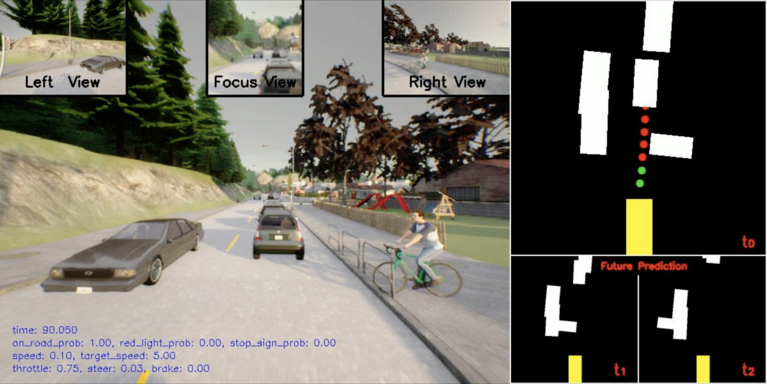
\includegraphics[width=\columnwidth]{images/RS01_R0_bikeRight.png}
        \Description{Initial situation with the cyclist stationary on the right side of the ego vehicle.}
        \caption{Initial scenario showing a stationary cyclist positioned on the sidewalk to the right of the ego vehicle (highlighted in red). Even though the cyclist is not moving, the InterFuser agent detects his presence and incorrectly forecasts his movement into the planned trajectory of the ego vehicle, creating a potential collision scenario.}
        \label{fig:RS01_initial_bike_right}
    \end{subfigure}
    \hfill
    \begin{subfigure}[b]{0.45\textwidth}
        \centering
        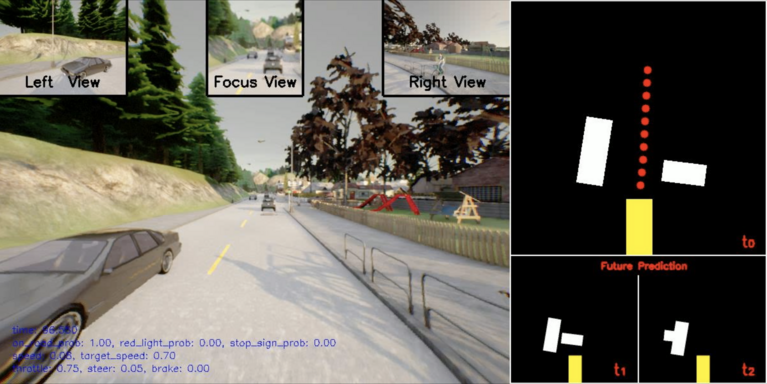
\includegraphics[width=\columnwidth]{images/RS01_R0_wrongPredBike.png}
        \Description{Incorrect predicted trajectory of the cyclist causing the InterFuser agent to remain stationary.}
        \caption{Incorrect trajectory prediction of the cyclist. This figure illustrates the incorrectly forecasted trajectory for the cyclist by InterFuser's tracking system (represented by the dashed line). Despite the cyclist remaining stationary throughout the observation period, the predicted trajectory continually intersects the ego vehicle's planned path, causing the vehicle to remain indefinitely stopped.}
        \label{fig:RS01_incorrect_bike_prediction}
    \end{subfigure}
    \caption{Illustrative example of the InterFuser agent being blocked due to its inability to accurately predict the future movements of a detected object located near the ego vehicle. Although the cyclist remains stationary and does not pose an actual threat, the incorrect movement prediction leads the system to adopt a conservative policy, indefinitely halting to avoid a perceived potential collision.}
    \label{fig:interfuser_prediction_issue}
\end{figure}

\begin{figure}[htbp]
    \centering
    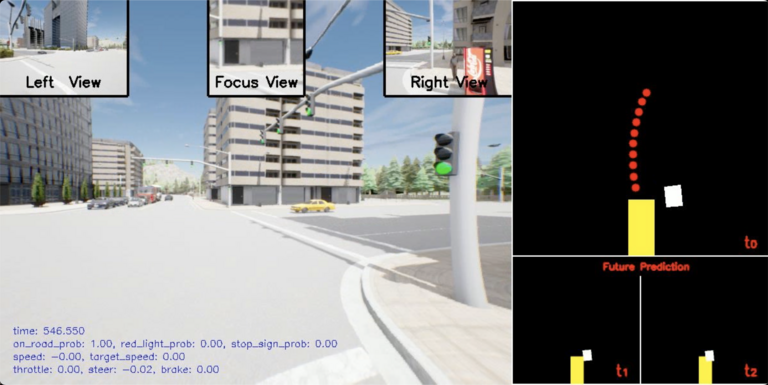
\includegraphics[width=\linewidth]{images/new_int_RS25.png}
    \Description{The InterFuser agent remains stationary due to a static Coca-Cola vending machine located to its right.}
    \caption{InterFuser agent immobilized due to erroneous collision risk assessment caused by a static Coca-Cola vending machine positioned to its right. Despite the object being clearly stationary and not posing a real threat, the system inaccurately predicts future movement into the ego vehicle’s planned trajectory, leading to indefinite vehicle blockage.}
    \label{fig:RS25_static_object_blocking}
\end{figure}

\subsection{P3. Agent Struggles in Very Dark Conditions}
\noindent\textbf{Issue.} In scenarios with extremely low lighting—such as night-time driving or poorly illuminated urban environments—the InterFuser agent exhibits noticeably degraded behavior. The vehicle struggles to detect and respond to environmental cues, including traffic lights, lane markings, pedestrians, and other vehicles. As a result, it may brake too late, swerve unexpectedly, or fail to react appropriately to dynamic objects on the road. These failures can lead to unsafe driving decisions and an overall drop in navigation performance.

\noindent\textbf{Reason.} The root cause of this problem lies primarily in the limitations of RGB-based perception under low-light conditions. The RGB cameras suffer from reduced visibility in the dark, resulting in poor detection of critical features necessary for navigation. Although the InterFuser agent also uses LiDAR—which is unaffected by lighting—its sensor fusion process relies heavily on information from RGB images. Consequently, when the camera data becomes unreliable, the entire perception and decision-making pipeline is compromised. Furthermore, it's likely that the model was not sufficiently trained on diverse nighttime scenarios, making it less robust to such environments.

\noindent\textbf{Proposed Solution.} To address this limitation, a two-pronged strategy can be employed. First, the model should be retrained or fine-tuned on more diverse datasets that include a substantial number of nighttime and low-light scenes. This would improve its ability to generalize across a wider range of lighting conditions.

Second, the sensor fusion architecture itself could be improved to better leverage LiDAR data when RGB inputs are degraded. One promising approach is to dynamically adjust the weighting of different sensor modalities depending on environmental context—i.e., relying more on LiDAR features when RGB quality is poor. Alternatively, thermal cameras or event-based sensors could be introduced as additional modalities to supplement the system in dark scenarios.

\begin{figure}[htbp]
    \centering
    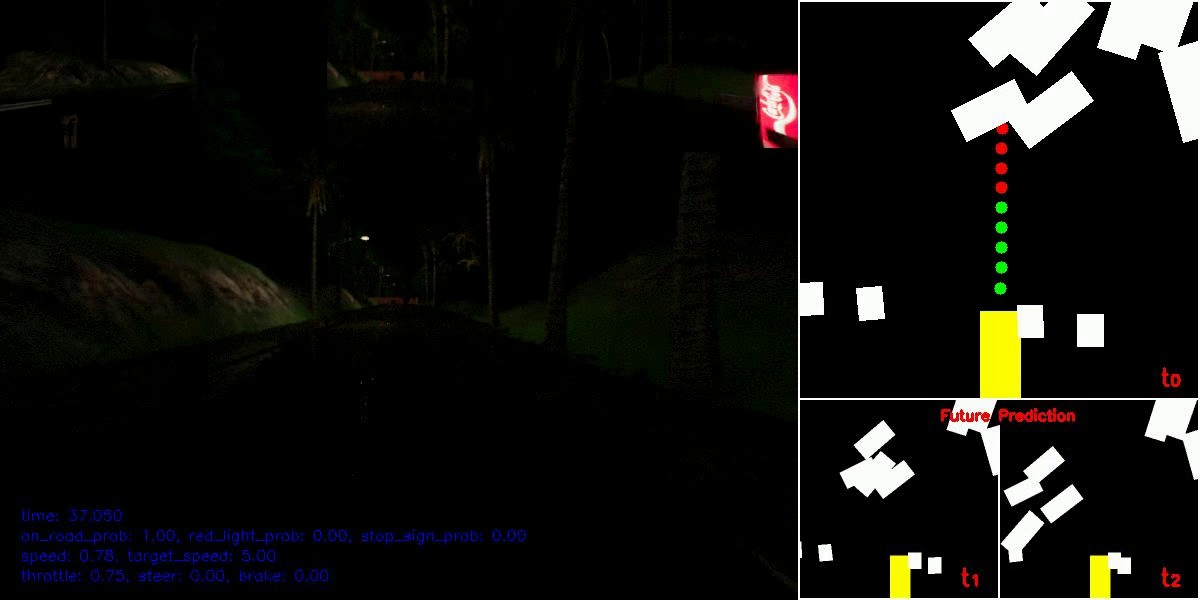
\includegraphics[width=\linewidth]{images/RS01_dark.png}
    \Description{RGB image captured in very low lighting conditions. Incorrect predictions by the InterFuser agent are visible through the displayed waypoints, which deviate from the correct trajectory.}
    \caption{Night-time scenario: the InterFuser agent generates incorrect predictions, failing to correctly identify the empty road due to poor lighting conditions.}
    \label{fig:dark_RS01}
\end{figure}

\begin{figure}[htbp]
    \centering
    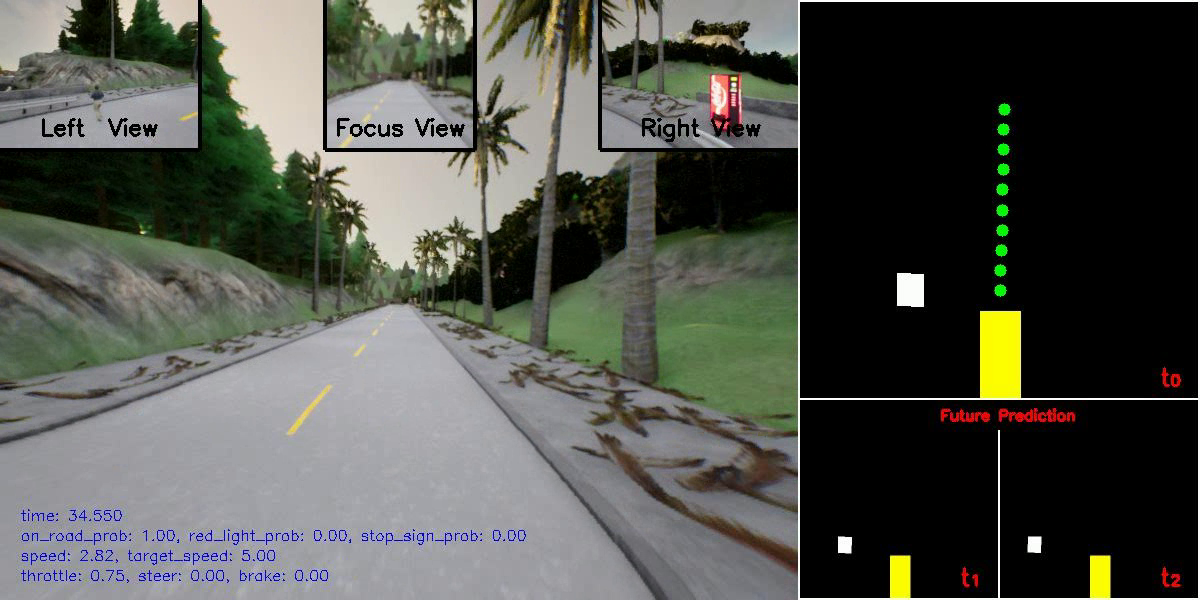
\includegraphics[width=\linewidth]{images/RS01_light.png}
    \Description{The same RGB image as the previous scenario, but under adequate lighting conditions. The waypoints predictions are accurate and closely follow the road trajectory.}
    \caption{Well-lit scenario: the InterFuser agent generates correct predictions, accurately identifying the clear road trajectory and ensuring safe navigation.}
    \label{fig:light_RS01}
\end{figure}

\subsection{P4. Car does not full stop at stop sign}
\noindent\textbf{Issue.} Simulation analysis revealed that the TransFuser agent occasionally fails to come to a complete stop at stop signs in certain scenarios. This behavior is also documented in the evaluation reports from the CARLA Leaderboard, which record specific violations for failing to comply with stop sign rules.

While the speed value may briefly drop to zero for a few frames, suggesting a momentary stop, in some instances, the agent continues through the intersection without fully halting, thereby breaching standard traffic regulations.

As shown in Figure~\ref{fig:tf_RS18_1}, the vehicle approaches the stop intersection with a speed greater than zero. A few frames later, as shown in Figure~\ref{fig:tf_RS18_2}, it can be seen that the car has passed through the intersection without braking or coming to a complete stop at the sign.

\noindent\textbf{Reason.} The stop sign detection logic in the TransFuser agent relies on proximity-based interaction with CARLA's stop sign actors. Specifically, the agent uses a bounding box intersection method to determine whether the ego vehicle's 3D bounding box intersects with the trigger volume of any nearby stop sign. These stop signs are detected using CARLA's actor filtering mechanism, where the code explicitly searches for actors with names containing the sub-string \textit{'*stop*'}.
Once nearby stop signs are identified (within a defined radius), the agent checks whether its own bounding box intersects the stop sign’s trigger volume. The trigger volume should represent the distance at which, if a stop is detected, the vehicle should stop. If an intersection is detected while the vehicle is moving (speed > 0), the stop sign is considered a hazard, and the brake will have to be activated. On the other side, if the vehicle is stationary at the time of intersection, the stop sign is marked as "cleared" and subsequent encounters with the same sign are ignored.

However, this logic could introduces some limitations:
\begin{itemize}
    \item\textbf{Reliance on proper actor placement}: the detection only works if a stop sign actor is present in the environment with a correctly placed and sized trigger volume. If the CARLA map omits the actor or misplaces the trigger, the agent will fail to recognize the intersection in the correct moment.
    \item\textbf{Temporal ambiguity in stopping logic}: even when a stop sign is detected, the agent only checks for momentary zero speed during the intersection period. If the vehicle briefly slows to zero (e.g. when it is in a queue of vehicles) but does not pause close to the stop sign line, it may incorrectly interpret this as a valid stop and continue forward, violating realistic traffic behavior.
    \item\textbf{No visual interpretation of road markings}: the system does not detect road text (e.g., the word \textit{STOP} painted on the asphalt, like in our case as we can see in Figure~\ref{fig:stop}), because such markings are not considered actors in CARLA and have no associated trigger volumes. If a stop location is indicated only via road paint, the vehicle will not recognize it as a stop sign, and therefore violate the intersection.
\end{itemize}

\begin{figure}[htbp]
    \centering
    \begin{subfigure}[b]{0.45\textwidth}
        \centering
        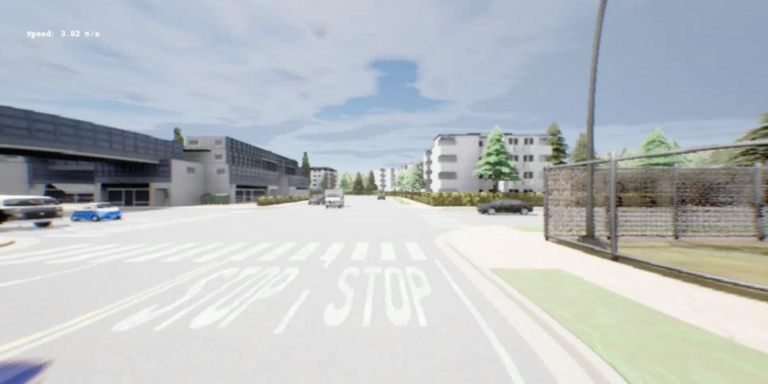
\includegraphics[width=\columnwidth]{images/RS18_noStopBefore.png}
        \Description{Transfuser vehicle approaches the stop sign}
        \caption{Vehicle approaching the stop}
        \label{fig:tf_RS18_1}
    \end{subfigure}
    \hfill
    \begin{subfigure}[b]{0.45\textwidth}
        \centering
        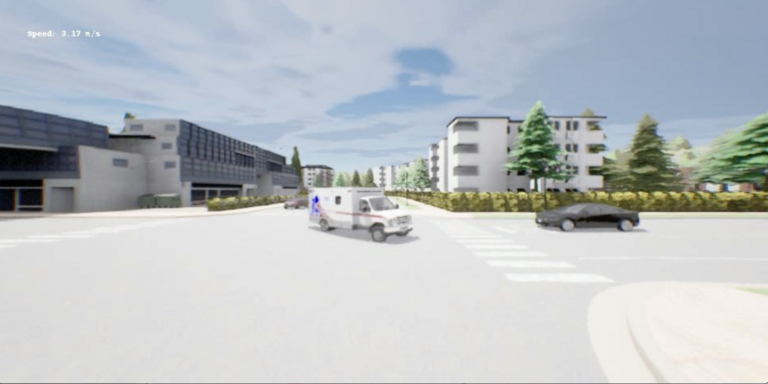
\includegraphics[width=\columnwidth]{images/RS18_noStopafter.png}
        \Description{Transfuser vehicle passes the stop sign without halting}
        \caption{After the stop}
        \label{fig:tf_RS18_2}
    \end{subfigure}
    \caption{Transfuser agent not recognizing the stop intersection and not halting.}
    \label{fig:stop}
\end{figure}

\noindent\textbf{Proposed Solution.} One possible solution is to supplement the current actor-based detection system with a visual analysis of the camera input. Specifically, the model can be extended to recognize the word “STOP” when it is painted on the road surface or on signs.

This could be done using a text recognition model (e.g., a small CNN trained to detect road text) applied to RGB cameras inputs. When the model detects the string “STOP” within a certain distance ahead of the vehicle, it can trigger the same stopping behavior used for stop sign actors. 
This visual detection would act as a complementary system to catch cases where a stop sign actor is missing or misplaced in the simulation and/or the intersection is marked only by road paint.
By combining both actor-based detection and visual stop word recognition, the agent would be more robust and better aligned with human driving behavior. This approach also brings the system one step closer to real-world perception, where traffic understanding is often based on a combination of signs, signals, and road markings.
For what concerns the issue where a stop intersection is prematurely marked as "cleared", the current logic considers a stop sign handled if the vehicle's speed reaches zero, even if only momentarily. This can result in the agent continuing through the intersection without performing a full stop, especially if the speed dips to zero for just a brief instant before accelerating again. 
To solve this, we propose adding a minimum stop duration threshold: when the vehicle enters a stop sign trigger volume (or detects a visual “STOP”), it must remain at 0 speed for a fixed amount of time — for example, 1.0 to 1.5 seconds — before proceeding. This ensures the stop is deliberate and complete, rather than a brief pause that doesn't meet traffic rules.

\subsection{P5. Can not see traffic lights turning green}
\noindent\textbf{Issue.} In some analyzed scenarios, the TransFuser agent was observed to stop prematurely, well before the designated stop line, when approaching traffic lights. As previously discussed in section \ref{P1}, this abnormal behavior—characterized by overly early stopping at intersections—negatively affects the agent’s ability to correctly interpret the traffic light’s status. As a result, the agent may fail to resume driving promptly, particularly in situations where the green phase is short, ultimately hindering overall navigation performance.

\noindent\textbf{Reason.} The primary cause of this issue lies in the excessive distance between the vehicle’s stopping position and the actual location of the traffic light. At such a distance, correctly identifying changes in the traffic light state (e.g., from red to green) becomes difficult, especially given that RGB camera images may lose crucial visual details at long range.

In particular, scenario evaluations revealed that when the vehicle stopped too far from the traffic light, it often failed to clearly perceive the light turning green. This led to delayed restarts, or in more severe cases, no restart at all—raising potential concerns for traffic flow and road safety.

\noindent\textbf{Proposed Solution.} A possible method to moderate this problem could be to implement a temporal smoothing mechanism for traffic light state detection. Instead of relying only on the current rgb frame to determine the traffic light status, the agent could aggregate recent observations over several frames to better infer when a light has turned green. This would help reduce missed detections caused by stopping at a distance where the light is less visible in individual frames.

\begin{figure}[htbp]
    \centering
    \begin{subfigure}[t]{1\columnwidth}
        \centering
        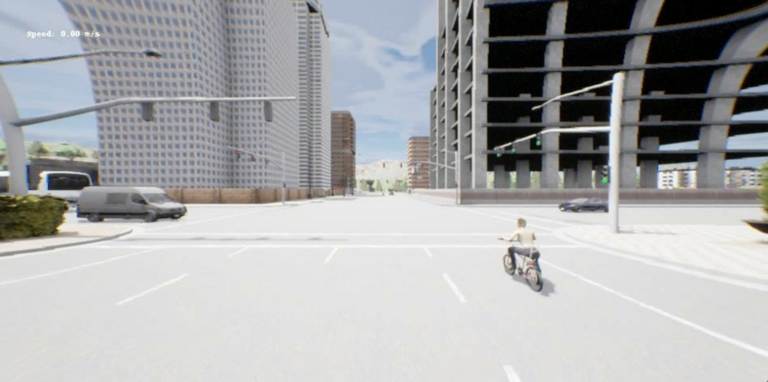
\includegraphics[width=\linewidth]{images/RS18_stopsFar.png}
        \Description{TransFuser vehicle stops prematurely at an excessive distance from the intersection, compromising visibility of the traffic light state.}
        \caption{TransFuser vehicle prematurely stops significantly far from the intersection and the traffic light. The substantial distance between the stopping position and the traffic signal reduces the agent's ability to accurately perceive traffic light state changes, particularly transitions from red to green, due to limited visual clarity at long distances.}
        \label{fig:tf_tlight_premature_stop}
    \end{subfigure}
    \hfill
    \begin{subfigure}[t]{1\columnwidth}
        \centering
        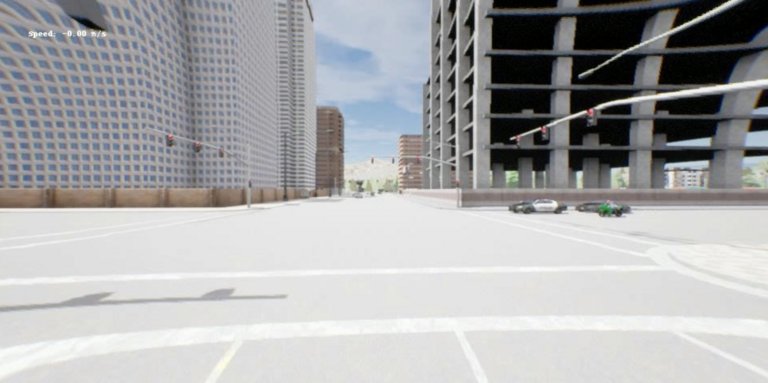
\includegraphics[width=\linewidth]{images/RS18_closer.png}
        \Description{TransFuser vehicle advances closer to the traffic signal, thus improving its visibility of the traffic light state.}
        \caption{TransFuser vehicle after advancing closer to the intersection and the traffic signal. The reduced distance considerably enhances the visibility of the traffic light, enabling the agent to correctly identify state transitions (e.g., from red to green) and respond more promptly, thus improving navigation efficiency.}
        \label{fig:tf_tlight_better_position}
    \end{subfigure}
    \hfill
    \begin{subfigure}[t]{1\columnwidth}
        \centering
        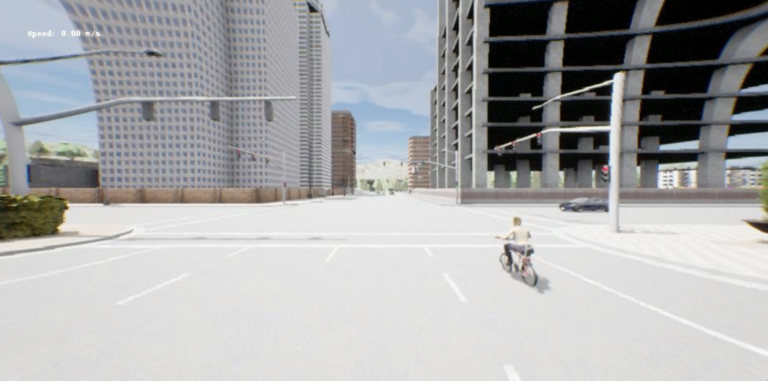
\includegraphics[width=\columnwidth]{images/RS18_green.png}
        \Description{The TransFuser vehicle fails to clearly perceive the green traffic signal due to excessive stopping distance.}
        \caption{TransFuser vehicle unable to perceive the traffic light's transition to green due to excessive distance from the intersection. The substantial gap between the vehicle and the traffic signal prevents the agent from effectively recognizing when the red light changes to green, causing unnecessary delays or potentially complete failure to resume driving promptly.}
        \label{fig:tf_unseen_greenlight}
    \end{subfigure}
    \caption{Illustrative example of the TransFuser agent's problematic behavior at traffic-controlled intersections. Initial premature stopping, as shown in (a), negatively impacts the vehicle’s ability to accurately detect traffic light state changes. When positioned closer, as shown in (b), the visibility and the ability to promptly respond to the traffic light significantly improves.}
    \label{fig:far_from_light}
\end{figure}

\subsection{P6. The problem of creeping}
\noindent\textbf{Issue.} In several evaluated scenarios, the TransFuser agent demonstrates unsafe behavior triggered by its built-in “creeping” mechanism. While the goal of this behavior is to overcome inertia in situations where the vehicle remains stationary for too long, in practice, it often activates in contexts where the ego vehicle is correctly stopped—such as when waiting at a red light or when blocked by other traffic participants. In these cases, the creeping behavior leads the agent to move forward inappropriately, occasionally resulting in collisions with nearby vehicles or cyclists.

This behavior is particularly problematic in crowded urban environments like \textit{Town05}, where the agent frequently misjudges whether the path ahead is truly clear. We observed multiple cases where creeping was activated despite the presence of surrounding traffic, leading the vehicle to either bump into other agents or be unable to brake in time.

\noindent\textbf{Reason.} The root cause of this issue lies in how the creeping behavior—referred to in the code as \textit{forced move}—is implemented in TransFuser. To counteract the tendency for the model to remain stuck due to learned patterns from training data (where a stationary vehicle often remains stationary), the authors introduced a strategy that triggers motion after the vehicle has been stopped for a prolonged period. Specifically, if the ego vehicle has been stationary for more than 550 frames, a creeping maneuver is activated by setting the PID controller's target speed to 4 m/s.

To avoid unsafe activation, the system includes a safety heuristic: it checks for obstacles in front of the vehicle using LiDAR data. If hits are detected within a predefined safety rectangle surrounding the ego vehicle, the creeping command is suppressed. However, this safety check has limitations. LiDAR sensors often have a minimum detection range, and objects within this range may not be detected. This can result in false negatives, causing the system to believe the area ahead is clear even when it isn’t.

In one analyzed scenario, a cyclist was directly in front of the ego vehicle, but the forced move was still activated due to a failure in obstacle detection—leading to a collision, as shown in Figure~\ref{fig:tf_forced}. In many other cases, the vehicle was reasonably distanced from the car ahead, yet the safety check passed due to the narrow rectangle used for LiDAR checks, again leading to unintended creeping and eventual crashes.

\begin{figure}[htbp]
    \centering
    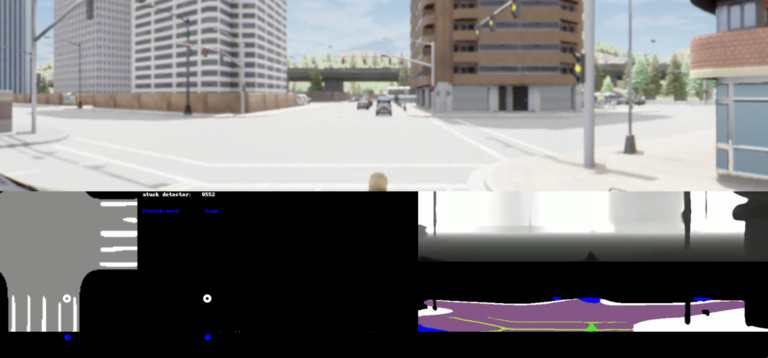
\includegraphics[width=\columnwidth]{images/RS23_forcedTF.png}
    \Description{TransFuser agent triggers the forced move behavior due to prolonged stationary period, despite an obstacle ahead.}
    \caption{TransFuser agent activating the forced move mechanism after remaining stationary for an extended period. This behavior, designed to overcome inertia, is triggered even though a cyclist is present directly in front of the vehicle, highlighting limitations in the LiDAR-based obstacle detection heuristic.}
    \label{fig:tf_forced}
\end{figure}

These situations are frequent, particularly in traffic-dense maps like \textit{Town05}, where minor misjudgments in space and timing can easily lead to accidents. Figure~\ref{fig:tf_forced_collision} shows a clear example: the vehicle initiates creeping when the forced move flag becomes true (left), and shortly after, collides with the car in front (right). Several similar collisions are reported in the final evaluation logs for this same scenario, all traced back to faulty creeping behavior.

\begin{figure}[htbp]
    \centering
    \begin{subfigure}[b]{0.45\textwidth}
        \centering
        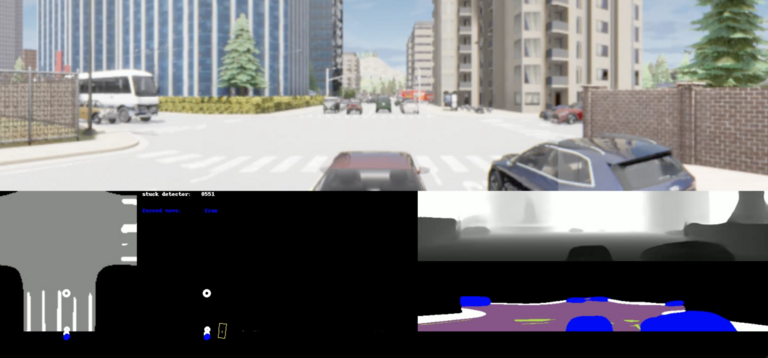
\includegraphics[width=\columnwidth]{images/RS23_official_forced.png}
        \Description{TransFuser agent stationary in traffic, forced move flag activates due to extended waiting period.}
        \caption{Forced move activated}
        \label{fig:tf_forced_collision_a}
    \end{subfigure}
    \hfill
    \begin{subfigure}[b]{0.45\textwidth}
        \centering
        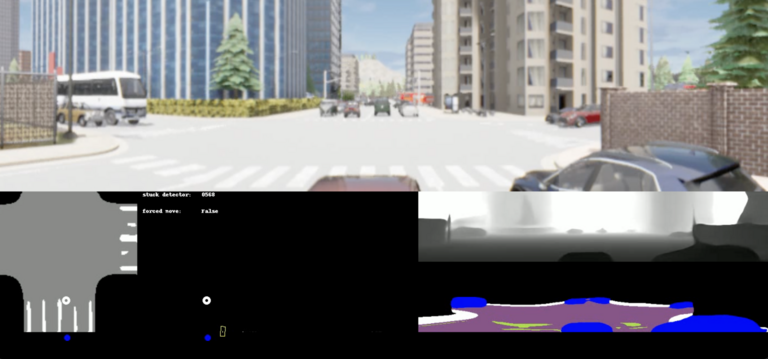
\includegraphics[width=\columnwidth]{images/RS23_official_collisionforced.png}
        \Description{TransFuser agent collides with vehicle in front after creeping forward.}
        \caption{Resulting collision}
        \label{fig:tf_forced_collision_b}
    \end{subfigure}
    \caption{Illustration of the TransFuser agent's problematic creeping behavior. After remaining stationary for a prolonged period, the forced move mechanism is triggered (a), causing the agent to creep forward erroneously and subsequently collide with the vehicle directly ahead (b). This incident underscores deficiencies in the LiDAR-based safety heuristic used to validate creeping.}
\label{fig:tf_forced_collision}
\end{figure}

\paragraph{\textbf{LatentTF}}
In contrast, the LatentTF model, which does not rely on LiDAR data, uses camera-based perception to detect surrounding vehicles. Its safety heuristic checks for intersections between a rectangular safety area around the ego vehicle and the bounding boxes of nearby objects. If no intersections are found, creeping is allowed.

In our experiments, LatentTF demonstrated better handling of creeping in traffic. For instance, in a dense traffic scenario where the vehicle exceeded the stationary time threshold, creeping was initiated. However, upon detecting a nearby vehicle using bounding box overlap from the camera feed, the agent immediately braked, avoiding a collision. Figures~\ref{fig:latent_forcedmove_a} and \ref{fig:latent_forcedmove_b} illustrate this behavior.

\begin{figure}[htbp]
    \centering
    \begin{subfigure}[b]{0.45\textwidth}
        \centering
        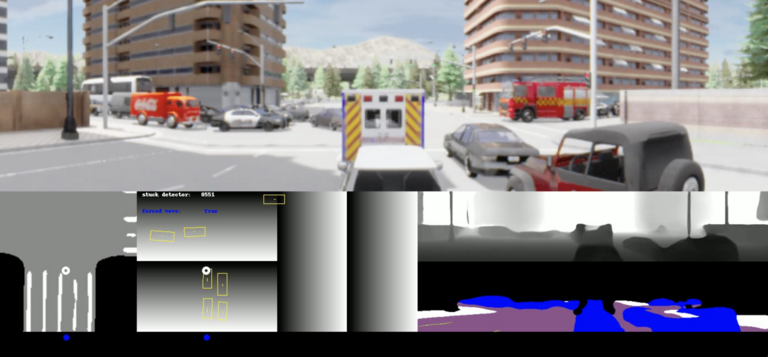
\includegraphics[width=\columnwidth]{images/latend_forced1.png}
        \Description{LatentTF agent stationary in dense traffic, triggering the forced move after a long waiting period.}
        \caption{Forced move activated}
        \label{fig:latent_forcedmove_a}
    \end{subfigure}
    \hfill
    \begin{subfigure}[b]{0.45\textwidth}
        \centering
        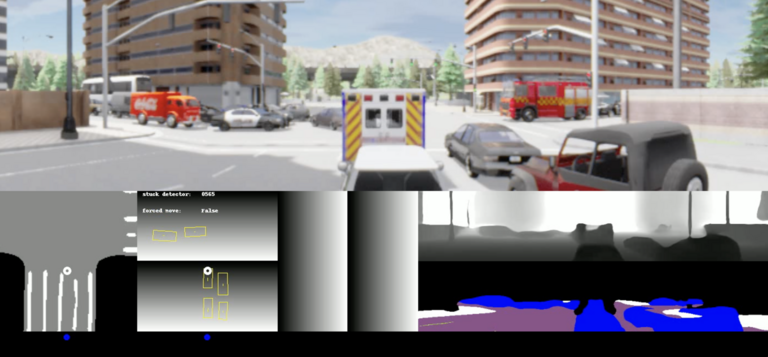
\includegraphics[width=\columnwidth]{images/latent_forced2.png}
        \Description{LatentTF agent creeps forward cautiously but promptly halts upon detecting a nearby obstacle.}
        \caption{Agent stops promptly}
        \label{fig:latent_forcedmove_b}
    \end{subfigure}
    \caption{Illustration of safer creeping behavior demonstrated by the LatentTF agent. Although initially triggering the forced move due to an extended stationary period (a), the camera-based bounding-box safety heuristic promptly identifies a nearby vehicle, causing the agent to halt before collision (b).}
    \label{fig:latent_forced}
\end{figure}

LatentTF appears more cautious in densely populated environments, leading to fewer collisions. Nevertheless, according to the original benchmark results, TransFuser still outperforms LatentTF on average across more diverse weather, towns, and scenario configurations.

\noindent\textbf{Proposed Solution.} A simple but effective way to face this problem, could be to incorporate a short term memory in the safety heuristic. The limitation with LiDAR, is that it fails in detecting the presence of an obstacle when the ego vehicle is stopped too close to it. 

To reduce the occurrences of accidents caused by these type of problems, we propose maintaining a brief temporal buffer of recent LiDAR detections. If an obstacle was clearly detected in front of the vehicle shortly before it stopped, the system should conservatively assume that the obstacle is still present, resulting in the suppression of the forced move and waiting for another cycle of time.

The same idea can also be extended to the camera-based version (LatentTF). When bounding boxes from the camera detect a vehicle, pedestrian, or cyclist in close proximity to the ego vehicle, and that detection suddenly disappears, the agent should not immediately assume the path is clear. Instead, it should reference recent past frames: if the obstacle was visible just before vanishing, the system should treat the zone as occupied.

In general, this solution could be particularly effective for LiDAR-based safety heuristic, which we found more prone to accidents in these situations. 
Nonetheless, integrating temporal consistency into obstacle checks could improve reliability across both sensing modalities and reduce the likelihood of collisions in highly congested or visually ambiguous situations.

\section{Conclusion}
\label{sec:conclusion}

This paper presents a comparative evaluation of InterFuser and TransFuser, two state-of-the-art AI-based autonomous driving agents, within the CARLA simulation environment. The primary objective was to assess and contrast their performance and behavioral characteristics in diverse urban driving scenarios. Leveraging the standardized CARLA Leaderboard metrics, the study systematically analyzed aspects such as route completion, infraction rates, and driving safety. Additionally, qualitative video footage of the agents' driving sessions was reviewed to identify and characterize unusual or problematic behaviors not captured by quantitative metrics.

The evaluation revealed several common failure modes across both models, including premature stopping at intersections or traffic lights, failure to come to a complete stop at stop signs, becoming indefinitely blocked in the presence of nearby static or dynamic obstacles, severe degradation of performance under low-light conditions, unreliable or unsafe creeping behavior leading to collisions, and inadequate throttle control on upward slopes. The findings contribute to the broader effort of benchmarking autonomous driving policies in simulation and support the informed development of future sensor fusion architectures.

\balance

%%
%% The next two lines define the bibliography style to be used, and
%% the bibliography file.
\bibliographystyle{ACM-Reference-Format}
\interlinepenalty=10000
\bibliography{acmart}

\end{document}
\endinput
%%
%% End of file `sample-sigconf.tex'.
